%Do not change 
\documentclass[12pt, oneside]{article}
\usepackage{amssymb,amsmath}
\usepackage[margin=1in]{geometry}
\usepackage{textpos}
\usepackage{float}
%\usepackage{color}
\usepackage{graphicx}
\usepackage{tikz}
\usetikzlibrary{positioning}
\usepackage{tikz-3dplot}
\usepackage{pgfopts}
\usepackage{wasysym}
\usepackage{structuralanalysis}

% You may add the packages you need here
%TODO: remove some problems
%TODO: add compounding problems
%TODO: stress concentration ratio


\begin{document}
% Do not modify 


%Do not modify
\begin{textblock*}{4cm}(-1.7cm,-2.3cm)
\noindent {\scriptsize AE737 Spring 2016} 
\end{textblock*}

%Do not modify other than putting your name where stated
\begin{textblock*}{8cm}(12.5cm,-1cm)
\noindent {Name: } 
\end{textblock*}
%Do not modify other than typing your acknowledgement where stated
\begin{textblock*}{13.5cm}(-1.7cm,-1.8cm)
%\noindent \textit{\footnotesize Acknowledgement: Your acknowledgement for collaboration and other sources goes here. } 
\end{textblock*}

\vspace{1cm}

%Do not modify other than typing the homework number after #
\begin{center}
\textbf{\Large Homework 1}

\textbf{Due 2 Feb 2016}
\end{center}


%Rest should contain your solution for the homework. Feel free to improvise in ways that you believe make grading easier.
\begin{enumerate}

\begin{figure}[H]
	\item 
Define \emph{stress intensity}
\end{figure}


\begin{figure}[H]
	\item
\begin{enumerate}
	\item Determine the value of $K_I$ for a center-cracked panel with $W/2a = 5$ and a uniformly applied remote stress, $\sigma$.
	\item Determine the value of $K_I$ for an edge-cracked panel with $W/a = 5$ and a uniformly applied remote stress, $\sigma$.
	\item Compare these two results. Note that in both cases the panel width to crack length ratio is the same. Why do you think these results are different?
\end{enumerate}
\end{figure}

\begin{figure}[H]
	\item For the plate shown below, determine $K_I$ for the following conditions
	\begin{enumerate}
		\item There is a .085" thru crack on one side of the hole.
		\item There are .085" thru cracks on both sides of the hole.
		\item There is a quarter circular crack of .085" radius on one side of the hole.
	\end{enumerate}
	\centering
	\begin{tikzpicture}
	\draw (-2,3) -- (2,3) -- (2,-3) -- (-2,-3) -- (-2,3);
	\draw (0,0) circle (0.5cm);
	\draw (0.5,0) -- (1.0,0);
	\draw (-0.5,0) -- (-1.0,0);
	\draw[->] (0,3) -- (0,4) node[above] {10,000 lb.};
	\draw[->] (0,-3) -- (0,-4);
	\draw[->] (-0.5,-2) node at (0,-2) {7"} -- (-2,-2);
	\draw[->] (0.5,-2) -- (2,-2);
	\draw[->] (0.5,2) node[right] {.25"$\diameter$} -- (0,0.5); 
	\draw node at (4,0) {$t = 0.157 \text{in.}$};
	\end{tikzpicture}
	%\caption{Plate for Problem 3}
	\label{fig:problem3}
\end{figure}

\begin{figure}[H]
	\item The panel shown below has a semi-elliptical surface flaw. Determine the maximum value for $K_I$ if the normal stress in the crack opening direction is 17,700 psi.
	\centering
	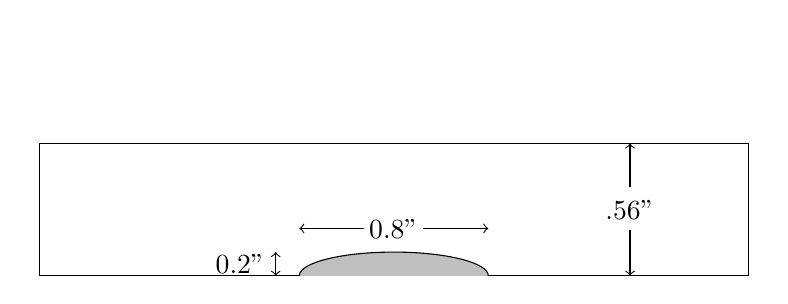
\begin{tikzpicture}
	\begin{scope}[rotate=90, scale=1.5]
	\clip (0,3.1) rectangle (2.1,-3.1);
	\draw (0,3) -- (1.12,3) -- (1.12,-3) -- (0,-3) -- (0,3);
	\draw[fill=gray!50] (0,0) ellipse [x radius=0.2, y radius=0.8];
	\draw[->] (0.75,-2) node at (.56,-2) {.56"} -- (1.12,-2); 
	\draw[->] (.39,-2) -- (0,-2);
	\draw[->] (0.4,-0.25) -- (0.4,-0.8) node at (0.4,0) {0.8"};
	\draw[->] (0.4,0.25) -- (0.4,0.8);
	\draw[<->] (0,1.0) -- (0.2,1.0);
	\draw node at (0.1, 1.3) {0.2"};
	\end{scope}
	\end{tikzpicture}
	%\caption{Plate for Problem 4}
	\label{fig:problem4}
\end{figure}

\begin{figure}[H]
	\item An aluminum beam has a 0.3" crack in the upper flange as shown. 
	Estimate the stress intensity.
	
	\centering
	\begin{minipage}{0.7\textwidth}
	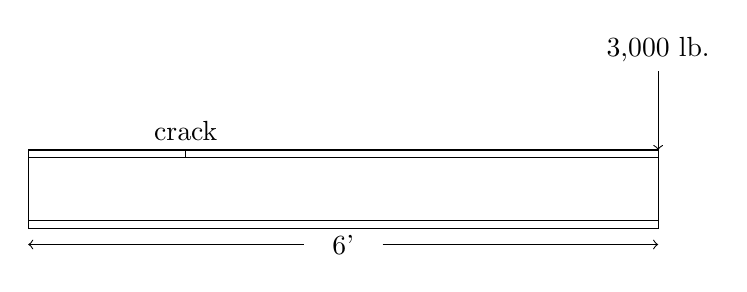
\begin{tikzpicture}
	\point{a}{0}{0};
	\draw (0,-0.5) -- (0,0.5) -- (8,0.5) -- (8,-0.5) -- (0,-0.5);
	\support{3}{a}[-90];
	\draw[->] (8,1.5) node[above] {3,000 lb.}--(8,0.5);
	\draw (0,0.4) -- (8,0.4);
	\draw (0,-0.4) -- (8,-0.4);
	\draw (2,0.5) node[above] {crack} -- (2,0.4);
	\draw[<-] (0,-0.7) -- (3.5,-0.7);
	\draw node at (4,-0.7) {6'};
	\draw[->] (4.5,-0.7) -- (8,-0.7);
	\end{tikzpicture}	
	\end{minipage}
	\begin{minipage}{0.25\textwidth}
		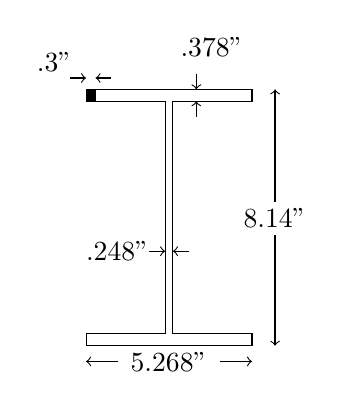
\begin{tikzpicture}
		\begin{scope}[scale=0.4]
		\draw (0,0) -- (5.268,0) -- (5.268, .378) -- (2.758,.378) -- (2.758, 7.762) -- (5.268, 7.762) -- (5.268, 8.14) -- (0,8.14) -- (0,7.762) -- (2.51,7.762) -- (2.51,.378) -- (0,.378) -- (0,0);
		\draw[fill=black] (0.3, 8.14) -- (0,8.14) -- (0,7.762) -- (0.3,7.762);
		\draw node at (2.634,-0.5) {5.268"};
		\draw[->] (1,-0.5) -- (0,-0.5);
		\draw[->] (4.268,-0.5) -- (5.268,-0.5);
		\draw node at (6,4.07) {8.14"};
		\draw[->] (6,3.507) -- (6,0);
		\draw[->] (6,4.57) -- (6,8.14);
		\draw node at (1,3) {.248"};
		\draw[->] (2,3) -- (2.51,3);
		\draw[->] (3.268,3) -- (2.758,3);
		\draw node at (4,9.5) {.378"};
		\draw[->] (3.5,8.64) -- (3.5,8.14);
		\draw[->] (3.5,7.262) -- (3.5,7.762);
		\draw node at (-1,9) {.3"};
		\draw[->] (-0.5,8.5) -- (0,8.5);
		\draw[->] (0.8,8.5) -- (0.3,8.5);
		\end{scope}
		\end{tikzpicture}
	\end{minipage}
	%\caption{Drawing for Problem 5}
\end{figure}

\begin{figure}[H]
	\item Estimate the stress intensity if the crack at the notch has a length $L$ of
	\begin{enumerate}
		\item 0.5"
		\item 0.025"
	\end{enumerate}
	The thickness is 0.375"
	
	\centering
	\begin{tikzpicture}
	\begin{scope}[scale=1.5]
	\point{a}{0}{2};
	\point{b}{6}{2};
	\point{c}{0}{-3};
	\point{d}{6}{-3};
	\draw (0,0.25) -- (0,1) -- (4,1) -- (4,-1) -- (0,-1) -- (0,-0.25);
	\draw (0,0.25) -- (0.1,0.25);
	\draw (0,-0.25) -- (0.1,-0.25);
	\draw (0.1,0.25) arc(90:-90:0.25);
	\draw (0.35,0) -- (0.85,0);
	\draw node at (0.1,0) {+};
	\draw[->] (-0.2,-0.5) -- (0,-0.5);
	\draw[->] (0.3,-0.5) -- (0.1,-0.5);
	\draw node at (-0.5,-0.5) {0.1"};
	\draw[->] (1.7,-0.7)--(0,-0.7);
	\draw[->] (2.3,-0.7) -- (4,-0.7);
	\draw node at(2,-0.7) {4"};
	\draw[->] (0.5,0.5) node[right]{0.25" R} -- (0.277,0.177);
	\draw node at (0.6,-0.2) {$L$};
	\draw[->] (0.45,-0.2) -- (0.35,-0.2);
	\draw[->] (0.75,-0.2) -- (0.85,-0.2);
	\lineload{3}{a}{b}[-.5][-.5];
	\draw node at (2,2) {$\sigma = 6000 \text{psi}$};
	\lineload{3}{c}{d}[.5][.5];
	\draw node at (2,-2) {$\sigma = 6000 \text{psi}$};
	\end{scope}
	\end{tikzpicture}
\end{figure}

\begin{figure}[H]
	\item A stiffened skin panel has a 10" crack between stiffeners as shown. The distance between stiffeners is 12", rivet pitch is 2", and tensile stress is 10 ksi.
	Skin thickness is 0.6" and stiffener cross sectional area is 3.1 in$^2$.
	Determine the stress intensity.
	
	How much do the stiffeners increase the strength?
	
	\textbf{Note:} In this problem, assume the edge effect for stiffeners is $\beta_S=0.9$
	
	\centering
	\begin{tikzpicture}
	\begin{scope}[scale=0.25]
	\point{a}{0}{1.5};
	\point{b}{10}{1.5};
	\point{c}{0}{-1.6};
	\point{d}{10}{-1.6};
	\draw (0,3) -- (40,3) -- (40,-3) -- (0,-3) -- (0,3);
	\draw (2,3) -- (3,3) -- (3,-3) -- (2,-3) -- (2,3);
	\draw (14,3) -- (15,3) -- (15,-3) -- (14,-3) -- (14,3);
	\draw (26,3) -- (27,3) -- (27,-3) -- (26,-3) -- (26,3);
	\draw (38,3) -- (39,3) -- (39,-3) -- (38,-3) -- (38,3);
	\lineload{3}{a}{b}[-2][-2];
	\draw node at (20,8) {$\sigma = 10 \text{ksi}$};
	\lineload{3}{c}{d}[2][2];
	\draw node at (20,-8) {$\sigma = 10 \text{ksi}$};
	\draw (16,0) -- (25,0);
	\draw node at (20.5,1) {$2a$};
	\draw (2.5,0) circle (0.15) (2.5,1)circle (0.15) (2.5,2)circle (0.15) (2.5,-2)circle (0.15) (2.5,-1)circle (0.15);
	\draw (14.5,0) circle (0.15) (14.5,1)circle (0.15) (14.5,2)circle (0.15) (14.5,-2)circle (0.15) (14.5,-1)circle (0.15);
	\draw (26.5,0) circle (0.15) (26.5,1)circle (0.15) (26.5,2)circle (0.15) (26.5,-2)circle (0.15) (26.5,-1)circle (0.15);
	\draw (38.5,0) circle (0.15) (38.5,1)circle (0.15) (38.5,2)circle (0.15) (38.5,-2)circle (0.15) (38.5,-1)circle (0.15);
	\end{scope}
	\end{tikzpicture}
\end{figure}

\begin{figure}[H]
	\item For the splice shown, use superposition and suggest a method to estimate the stress intensity at the corner crack.
	
	\centering
	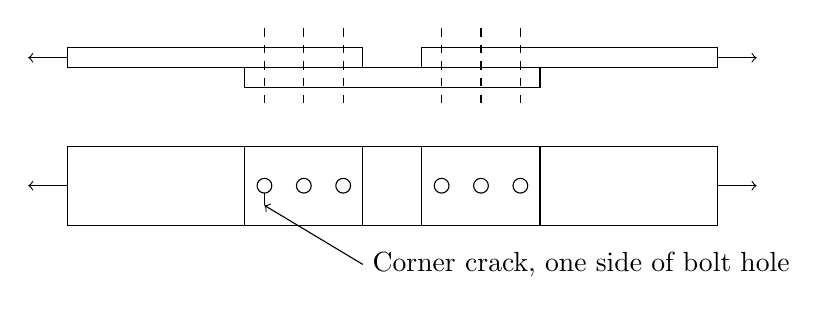
\begin{tikzpicture}
	\begin{scope}[scale=0.25]
	\draw (0,0) -- (0,1) -- (15,1) -- (15,0) -- (0,0);
	\draw (9,0) -- (24,0) -- (24,-1) -- (9,-1) -- (9,0);
	\draw (18,0) -- (18,1) -- (33,1) -- (33,0) -- (18,0);
	\draw[->] (0,0.5) -- (-2,0.5);
	\draw[->] (33,0.5) -- (35,0.5);
	\draw[dashed] (10,2) -- (10,-2);
	\draw[dashed] (12,2) -- (12,-2);
	\draw[dashed] (14,2) -- (14,-2);
	\draw[dashed] (19,2) -- (19,-2);
	\draw[dashed] (21,2) -- (21,-2);
	\draw[dashed] (23,2) -- (23,-2);
	\draw (0,-4) -- (0,-8) -- (15,-8) -- (15,-4) -- (0,-4);
	\draw (9,-4) -- (24,-4) -- (24,-8) -- (9,-8) -- (9,-4);
	\draw (18,-4) -- (18,-8) -- (33,-8) -- (33,-4) -- (18,-4);
	\draw[->] (0,-6) -- (-2,-6);
	\draw[->] (33,-6) -- (35,-6);
	\draw (10,-6) circle (0.375) (12,-6) circle (0.375) (14,-6) circle (0.375);
	\draw (19,-6) circle (0.375) (21,-6) circle (0.375) (23,-6) circle (0.375);
	\draw (10,-6.375) -- (10,-7);
	\draw[->] (15, -10) node[right] {Corner crack, one side of bolt hole} -- (10,-7);
	\end{scope}
	\end{tikzpicture}
\end{figure}

\begin{figure}[H]
	\item For the splice shown, estimate the stress intensity at the corner crack in the 2014-T6 plate.
	
	\centering
	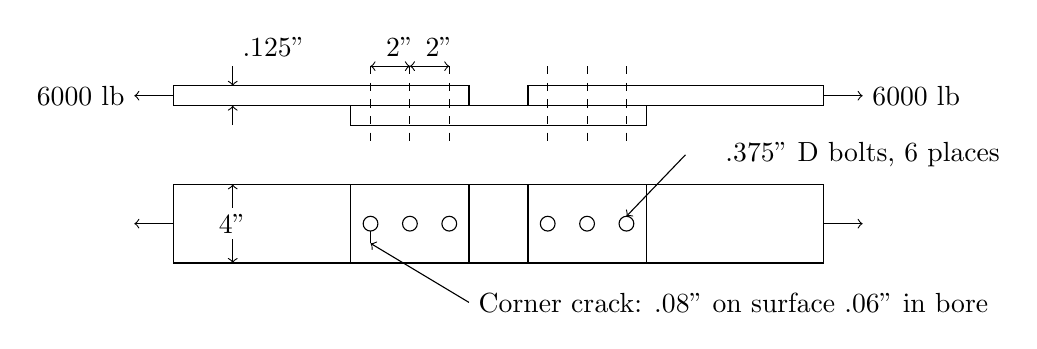
\begin{tikzpicture}
	\begin{scope}[scale=0.25]
	\draw (0,0) -- (0,1) -- (15,1) -- (15,0) -- (0,0);
	\draw (9,0) -- (24,0) -- (24,-1) -- (9,-1) -- (9,0);
	\draw (18,0) -- (18,1) -- (33,1) -- (33,0) -- (18,0);
	\draw[->] (0,0.5) -- (-2,0.5) node[left] {6000 lb};
	\draw[->] (33,0.5) -- (35,0.5) node[right] {6000 lb};
	\draw[->] (3,2) node[above right] {.125"} -- (3,1);
	\draw[->] (3,-5.2) -- (3,-4);
	\draw[->] (3,-6.8) -- (3,-8);
	\draw node at(3,-6) {4"};
	\draw[->] (3,-1) -- (3,0);
	\draw[dashed] (10,2) -- (10,-2);
	\draw[dashed] (12,2) -- (12,-2);
	\draw[dashed] (14,2) -- (14,-2);
	\draw[dashed] (19,2) -- (19,-2);
	\draw[dashed] (21,2) -- (21,-2);
	\draw[dashed] (23,2) -- (23,-2);
	\draw[<->] (10,2) -- (12,2);
	\draw[<->] (12,2) -- (14,2);
	\draw node at (11.5,3) {2"};
	\draw node at (13.5,3) {2"};
	\draw (0,-4) -- (0,-8) -- (15,-8) -- (15,-4) -- (0,-4);
	\draw (9,-4) -- (24,-4) -- (24,-8) -- (9,-8) -- (9,-4);
	\draw (18,-4) -- (18,-8) -- (33,-8) -- (33,-4) -- (18,-4);
	\draw[->] (0,-6) -- (-2,-6);
	\draw[->] (33,-6) -- (35,-6);
	\draw (10,-6) circle (0.375) (12,-6) circle (0.375) (14,-6) circle (0.375);
	\draw (19,-6) circle (0.375) (21,-6) circle (0.375) (23,-6) circle (0.375);
	\draw (10,-6.375) -- (10,-7);
	\draw[->] (15, -10) node[right] {Corner crack: .08" on surface .06" in bore} -- (10,-7);
	\draw node at (35,-2.5) {.375" D bolts, 6 places};
	\draw[->] (26,-2.5) -- (23,-5.625);
	\end{scope}
	\end{tikzpicture}
\end{figure}


\begin{figure}[H]
	\item Calculate the stress intensity in the splice plate shown, which is loaded by steel bolts at their single shear capacity of 4650 lbs. The plate has a thickness of 0.2" and a center crack of 0.49", with $\nu = 0.33$. Assume the plate is very wide relative to the other dimensions.
	
	\centering
	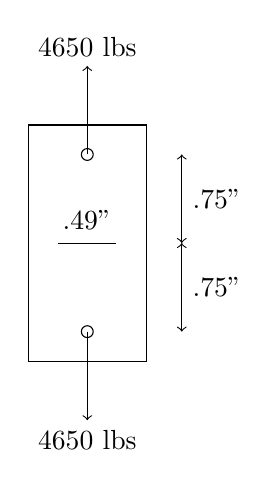
\begin{tikzpicture}
	\begin{scope}[scale=1.5]
	\draw (0,-1) -- (0,1) -- (1,1) -- (1,-1) -- (0,-1);
	\draw (0.255,0) -- (0.745,0);
	\draw (0.5,0.75) circle (0.05) (0.5,-0.75) circle (0.05);
	\draw node at (0.5,0.2) {.49"};
	\draw[->] (0.5,0.75) -- (0.5,1.5) node[above] {4650 lbs};
	\draw[->] (0.5,-0.75) -- (0.5,-1.5) node[below] {4650 lbs};
	\draw[<->] (1.3,0) -- (1.3,0.75);
	\draw[<->] (1.3,0) -- (1.3,-0.75);
	\draw node at (1.6,0.375) {.75"} node at (1.6,-0.375) {.75"};
	\end{scope}
	\end{tikzpicture}
\end{figure}

\begin{figure}[H]
	\item Determine the expression for stress intensity
	\begin{enumerate}
		\item In panel 1
		\item Use superposition to determine the stress intensity in panel 2
	\end{enumerate}
	
	\centering
	\begin{tikzpicture}
	\begin{scope}[scale=2]
	\point{a}{6}{-3.25};
	\point{b}{8}{-3.25};
	\draw (0,-1) -- (0,1) -- (1,1) -- (1,-1) -- (0,-1);
	\draw (0.3,0) -- (0.7,0);
	\draw[->] (0.5,0.2) -- (0.5,0.6) node[above] {P};
	\draw[->] (0.5,-0.2) -- (0.5,-0.6) node[below] {P};
	\draw node at (0.5,0.1) {$2a$};
	\draw (3,-1) -- (3,1) -- (4,1) -- (4,-1) -- (3,-1);
	\draw (3.3,0) -- (3.7,0);
	\draw[->] (3.5,0.2) -- (3.5,0.6) node[above] {P};
	\draw node at (3.5,-0.1) {$2a$};
	\lineload{3}{a}{b}[.25][.25];
	\draw node at (3.5,-1.5) {$\sigma$};
	\draw node at (0.5,1.5) {1};
	\draw node at (3.5,1.5) {2};
	\end{scope}
	\end{tikzpicture}
\end{figure}

\begin{figure}[H]
	\item Compare the stress intensities of the two cases where $2a = 2L + 2R$.
	
	\centering
	\begin{tikzpicture}
	\begin{scope}[scale=1.5]
	\draw (0,-1) -- (0,1) -- (2,1) -- (2,-1) -- (0,-1);
	\draw[->] (1,1) -- (1,1.2) node[above] {$\sigma$};
	\draw[->] (1,-1) -- (1,-1.2) node[below] {$\sigma$};
	\draw (1,0) circle(0.25);
	\draw (0.5,0) -- (0.75,0);
	\draw (1.25,0) -- (1.5,0);
	\draw (3,-1) -- (3,1) -- (5,1) -- (5,-1) -- (3,-1);
	\draw (3.5,0) -- (4.5,0);
	\draw[->] (4,1) -- (4,1.2) node[above] {$\sigma$};
	\draw[->] (4,-1) -- (4,-1.2) node[below] {$\sigma$};
	\draw node at (4,0.1) {$2a$};
	\draw node at (0.5,1.5) {1};
	\draw node at (3.5,1.5) {2};
	\draw node at (0.625,-0.2) {$L$};
	\draw node at (1.375,-0.2) {$L$};
	\draw node at (1,0.5) {$2R$};
	\draw[->] (1.4,0.5) -- (1.25,0.5);
	\draw[->] (0.6,0.5) -- (0.75,0.5);
	\end{scope}
	\end{tikzpicture}
\end{figure}

\begin{figure}[H]
	\item Determine the stress intensity for the panel shown
	
	\centering
	\begin{tikzpicture}
	\begin{scope}[scale=2]
	\point{a}{0}{-3.25};
	\point{b}{2}{-3.25};
	\point{c}{0}{2};
	\point{d}{2}{2};
	\draw (0,-1) -- (0,1) -- (1,1) -- (1,-1) -- (0,-1);
	\draw (0.3,0) -- (0.7,0);
	\draw[->] (0.5,0.2) -- (0.5,0.6) node[above] {P};
	\draw node at (0.5,-0.1) {$2a$};
	\lineload{3}{a}{b}[.25][.25];
	\lineload{3}{c}{d}[-.25][-.25];
	\draw node at (.5,-1.5) {$\sigma_2$};
	\draw node at (.5,1.5) {$\sigma_1$};
	\end{scope}
	\end{tikzpicture}
\end{figure}

\begin{figure}[H]
	\item The panel shown has a remote bypass stress of 5000 psi and a fastener load of 8000 lb/in. of thickness. Determine the stress intensity.
	
	\centering
	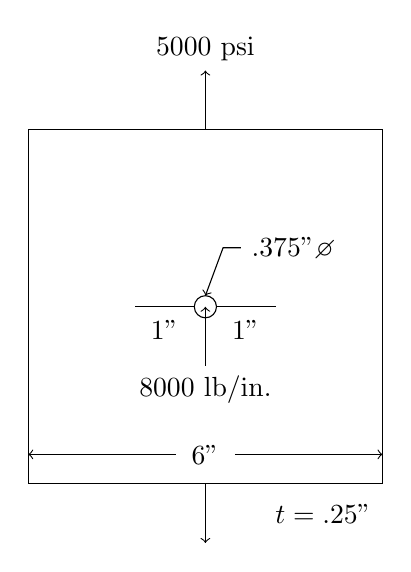
\begin{tikzpicture}
	\begin{scope}[scale=.75]
	\draw (0,-3) -- (0,3) -- (6,3) -- (6,-3) -- (0,-3);
	\draw[->] (3,3) -- (3,4) node[above] {5000 psi};
	\draw[->] (3,-3) -- (3,-4);
	\draw (3,0) circle (0.1875);
	\draw (3.1875,0) -- (4.1875,0);
	\draw (2.8125,0) -- (1.8125,0);
	\draw node at (3.6875,-0.4) {1"};
	\draw node at (2.3125,-0.4) {1"};
	\draw node at (4.5,1) {.375"$\diameter$};
	\draw[->] (3.6,1) -- (3.3,1) -- (3,.1875);
	\draw[->] (3,-1) node[below] {8000 lb/in.} -- (3,0);
	\draw[->] (2.5,-2.5) -- (0,-2.5);
	\draw[->] (3.5,-2.5) -- (6,-2.5);
	\draw node at (3,-2.5) {6"};
	\draw node at (5,-3.5) {$t=.25$"};
	\end{scope}
	\end{tikzpicture}
\end{figure}

\begin{figure}[H]
	\item Quite often, and sometimes in poor judgment, the expression
	\begin{equation*}
	K_I = 1.12 \sigma \sqrt{\pi a}
	\end{equation*}
	is used for the configuration shown, where 1.12 is called the back surface correction. Determine the stress intensity for
	\begin{enumerate}
		\item $K_I=1.12 \sigma \sqrt{\pi a}$
		\item $K_I=\sigma \sqrt{\pi a} \beta$
	\end{enumerate}
	and compare results.
	
	\centering
	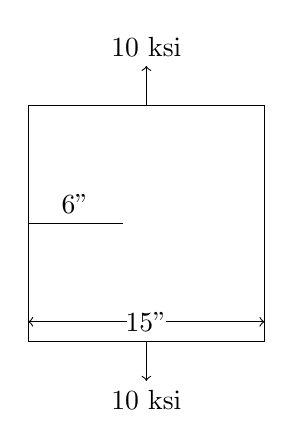
\begin{tikzpicture}
	\begin{scope}[scale=.5]
	\draw (0,-3) -- (0,3) -- (6,3) -- (6,-3) -- (0,-3);
	\draw[->] (3,3) -- (3,4) node[above] {10 ksi};
	\draw[->] (3,-3) -- (3,-4) node[below] {10 ksi};
	\draw (0,0) -- (2.4,0);
	\draw node at (1.2,0.5) {6"};
	\draw[->] (2.5,-2.5) -- (0,-2.5);
	\draw[->] (3.5,-2.5) -- (6,-2.5);
	\draw node at (3,-2.5) {15"};
	\end{scope}
	\end{tikzpicture}
\end{figure}

\begin{figure}[H]
	\item Determine the stress intensity if:
	\begin{enumerate}
		\item The crack is a thru crack
		\item The crack is a quarter circular corner crack
	\end{enumerate}
	
	\centering
	\centering
	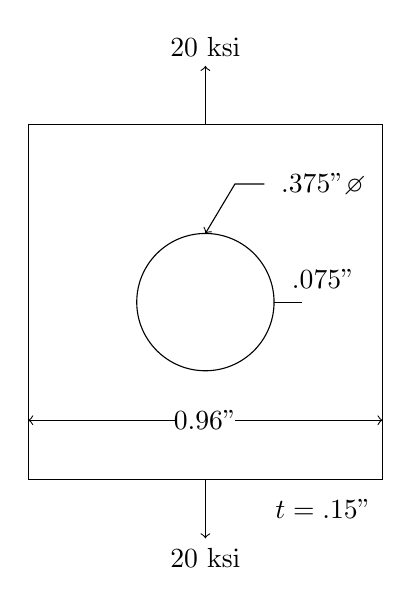
\begin{tikzpicture}
	\begin{scope}[scale=.75]
	\draw (0,-3) -- (0,3) -- (6,3) -- (6,-3) -- (0,-3);
	\draw[->] (3,3) -- (3,4) node[above] {20 ksi};
	\draw[->] (3,-3) -- (3,-4) node[below] {20 ksi};
	\draw (3,0) circle (1.1625);
	\draw (4.1625,0) -- (4.63125,0);
	\draw node at (5,0.4) {.075"};
	\draw node at (5,2) {.375"$\diameter$};
	\draw[->] (4,2) -- (3.5,2) -- (3,1.1625);
	\draw[->] (2.5,-2) -- (0,-2);
	\draw[->] (3.5,-2) -- (6,-2);
	\draw node at (3,-2) {0.96"};
	\draw node at (5,-3.5) {$t=.15$"};
	\end{scope}
	\end{tikzpicture}
\end{figure}

\begin{figure}[H]
	\item Use superposition to derive the expression for stress intensity for the case shown. There is a fastener load at the hole and the hole is small compared to the crack length.
	
	\centering
	\begin{tikzpicture}
	\begin{scope}[scale=.75]
	\draw (0,-3) -- (0,3) -- (6,3) -- (6,-3) -- (0,-3);
	\draw[->] (3,-3) -- (3,-4) node[below] {$\sigma$};
	\draw[->] (3,0) -- (3,1) node[above] {$P = \sigma Wt$};
	\draw node at (3,-0.5) {$2a$};
	\draw[->] (2.5,-0.5) -- (1.5,-0.5);
	\draw[->] (3.5,-0.5) -- (4.5,-0.5);
	\draw (3,0) circle (0.05);
	\draw (3.05,0) -- (4.5,0);
	\draw (2.95,0) -- (1.5,0);
	\end{scope}
	\end{tikzpicture}
\end{figure}

\end{enumerate}
\end{document}
